\documentclass{article}

%Preamble
\title{CS 585 Assignment 2}
\author{Don Johnson}
\date{January 29, 2014}
\usepackage{graphicx}
\usepackage[margin=0.5in]{geometry}
\usepackage{listings}
\lstset{language=C}
\usepackage{caption}
\usepackage{subcaption}
\usepackage{underscore}
\usepackage{mathtools}
\usepackage{float}

%Content
\begin{document}
\maketitle
\section{Assignment 2 (100 points)}
\subsection{Learning Objectives}
\subsection{Technical Task (30 points)}
Source code for technical task in ZIP file: Assignment2.cpp, Assignment2.hpp, Gui.cpp and Operators.cpp. All output images are in a subfolder in the ZIP file called "assignment2/Data."

\subsection{Programming Assignment Questions (28 points)}

\begin{enumerate}

\item
Run your program on the image yellowEgg.jpg both by thresholding the gradient magnitude and by using the Canny edge detector. Choose a threshold and smoothing level that leads to a nice contour and filled region of the egg. Results below:

Note: Smoothing value units are one standard deviation and threshold values are pixel integer values. Unlike the gradient edge detector, the Canny has both a lower and upper threshold that I set to be threes times the lower threshold. Consequently, the Canny output files have two thresholds in their name.

\begin{figure}[!htbp]
\centering
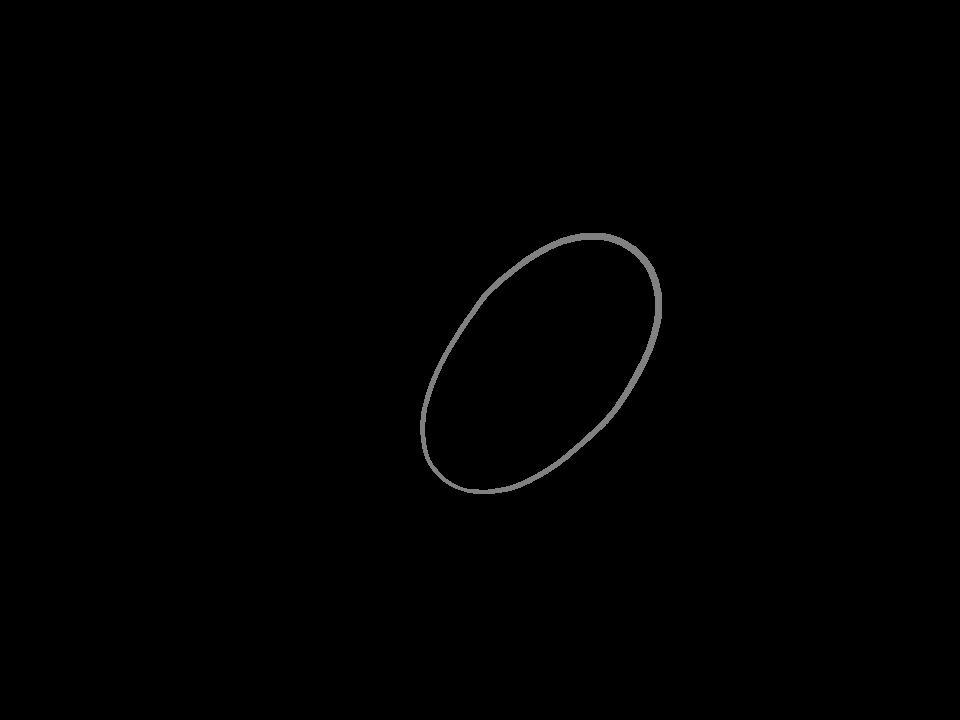
\includegraphics[width=140mm]{/Users/donj/workspace/cs585/Lab2/Mac/Assignment2/Data/SoloYellowEgg-Gradient-edges-2pt5-82.png}
\caption{SoloYellowEgg-Gradient-edges-2pt5-82.png}
\label{overflow}
\end{figure}

\begin{figure}[H]
\centering
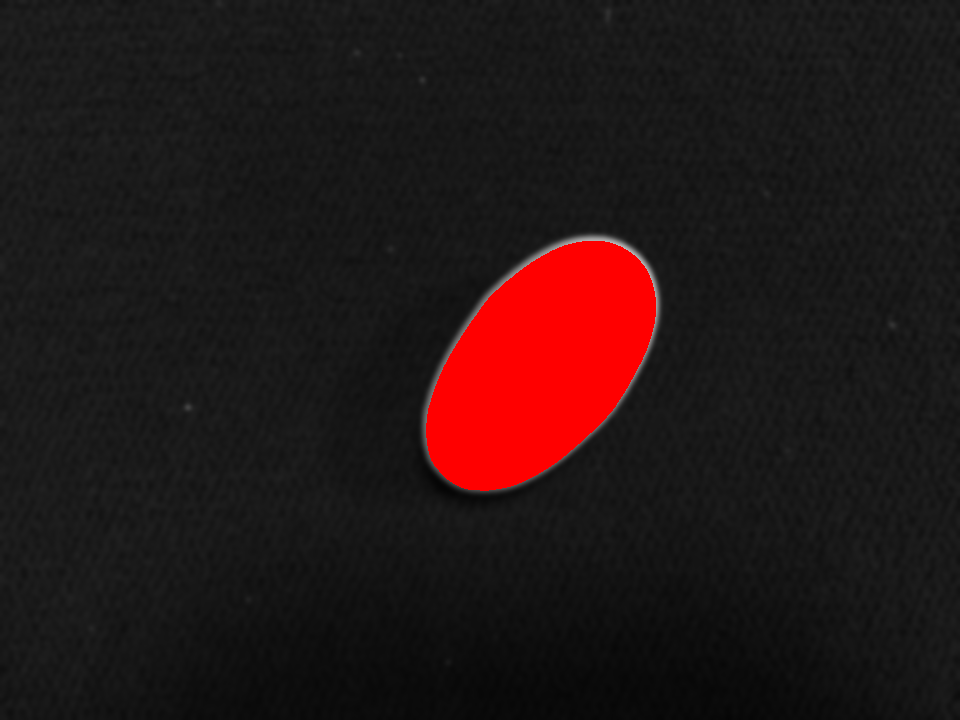
\includegraphics[width=140mm]{/Users/donj/workspace/cs585/Lab2/Mac/Assignment2/Data/SoloYellowEgg-Gradient-result-2pt5-82.png}
\caption{SoloYellowEgg-Gradient-result-2pt5-82.png}
\label{overflow}
\end{figure}

\begin{figure}[H]
\centering
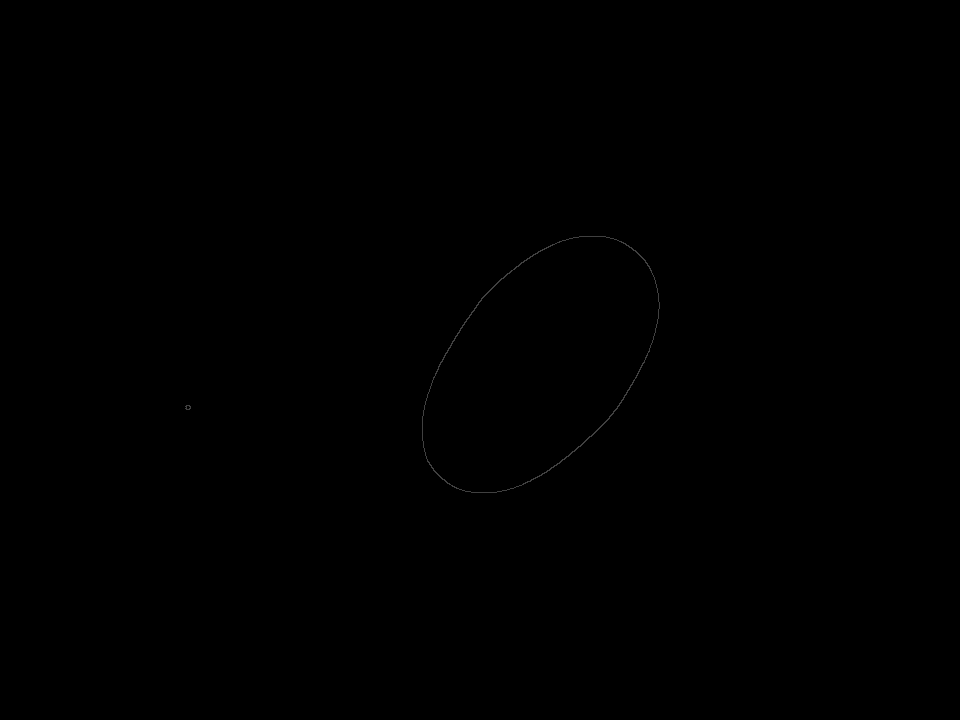
\includegraphics[width=140mm]{/Users/donj/workspace/cs585/Lab2/Mac/Assignment2/Data/SoloYellowEgg-Canny-edges-1-129-387.png}
\caption{SoloYellowEgg-Canny-edges-1-129-387.png}
\label{overflow}
\end{figure}

\begin{figure}[H]
\centering
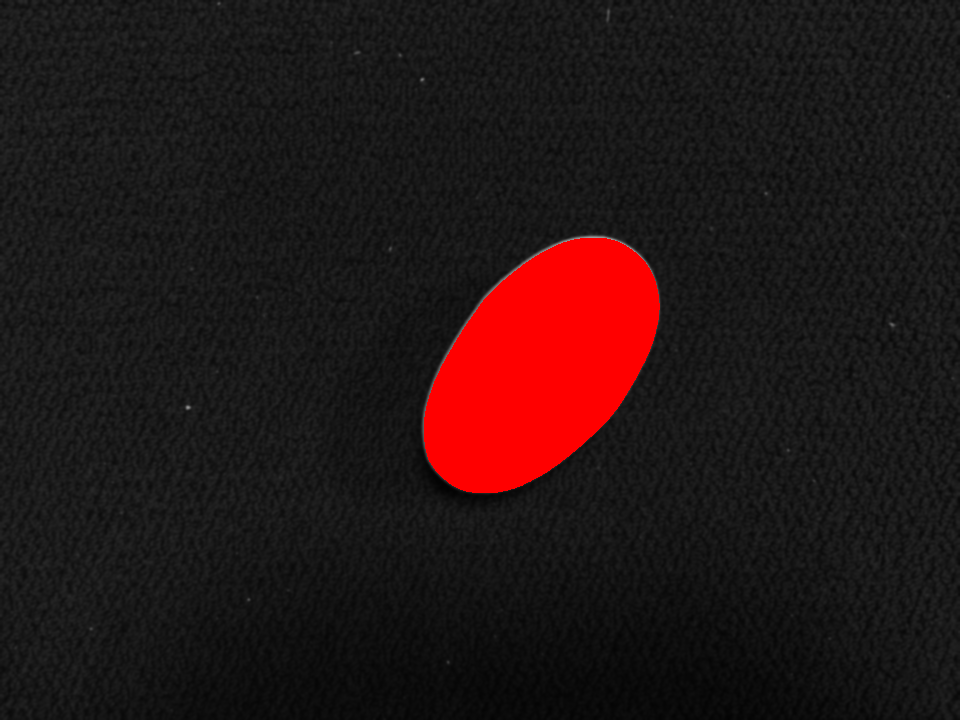
\includegraphics[width=140mm]{/Users/donj/workspace/cs585/Lab2/Mac/Assignment2/Data/SoloYellowEgg-Canny-result-1-129-387.png}
\caption{SoloYellowEgg-Canny-result-1-129-387.png}
\label{overflow}
\end{figure}

\item
Run your program on the image "eggsAndCube.jpg." Choose a smoothing level that you feel gives good contours in the gradient magnitude, and then for each of the red, green, blue, and yellow eggs, choose the highest threshold that gives a clean result. Results below:

\begin{figure}[H]
\centering
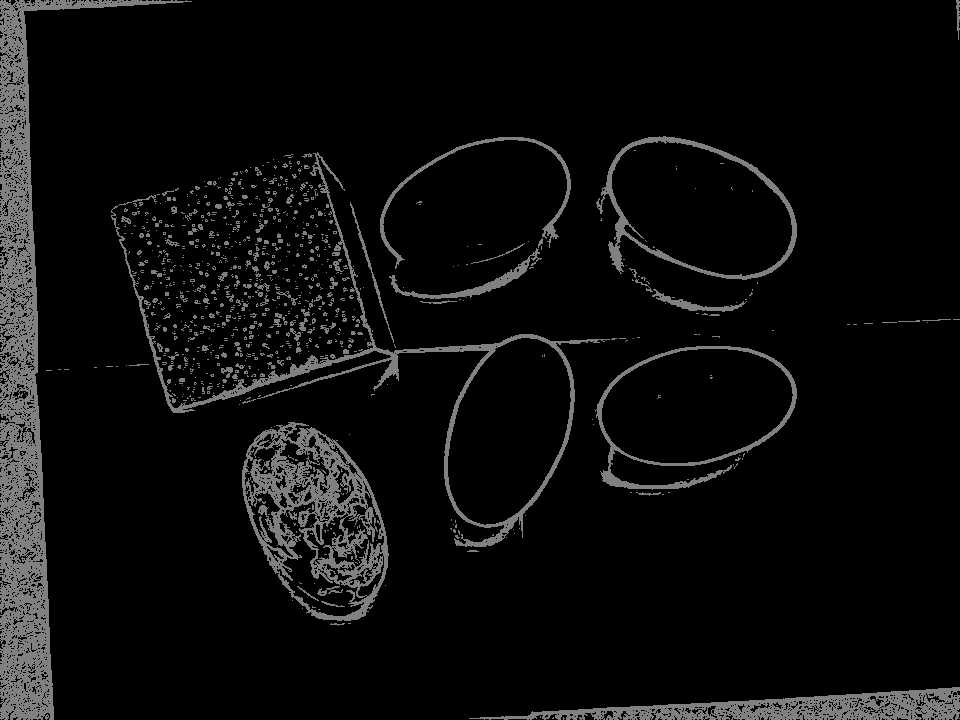
\includegraphics[width=140mm]{/Users/donj/workspace/cs585/Lab2/Mac/Assignment2/Data/redEgg-edges-0pt5-41.png}
\caption{redEgg-edges-0pt5-41.png}
\label{overflow}
\end{figure}

\begin{figure}[H]
\centering
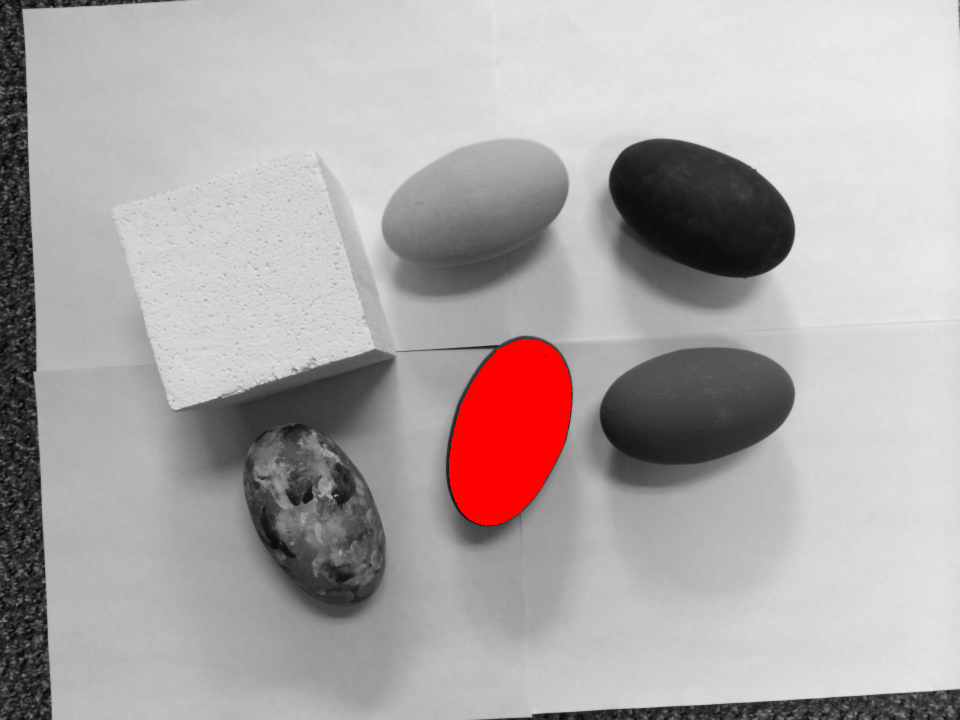
\includegraphics[width=140mm]{/Users/donj/workspace/cs585/Lab2/Mac/Assignment2/Data/redEgg-result-0pt5-41.png}
\caption{redEgg-result-0pt5-41.png}
\label{overflow}
\end{figure}

\begin{figure}[H]
\centering
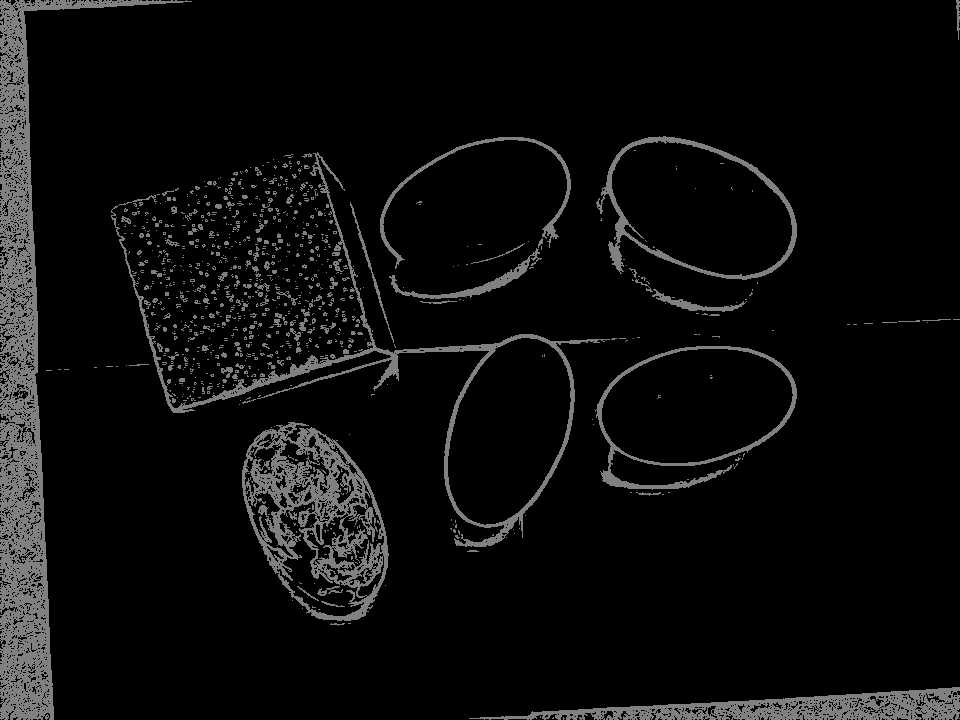
\includegraphics[width=140mm]{/Users/donj/workspace/cs585/Lab2/Mac/Assignment2/Data/greenEgg-edges-0pt5-41.png}
\caption{greenEgg-edges-0pt5-41.png}
\label{overflow}
\end{figure}

\begin{figure}[H]
\centering
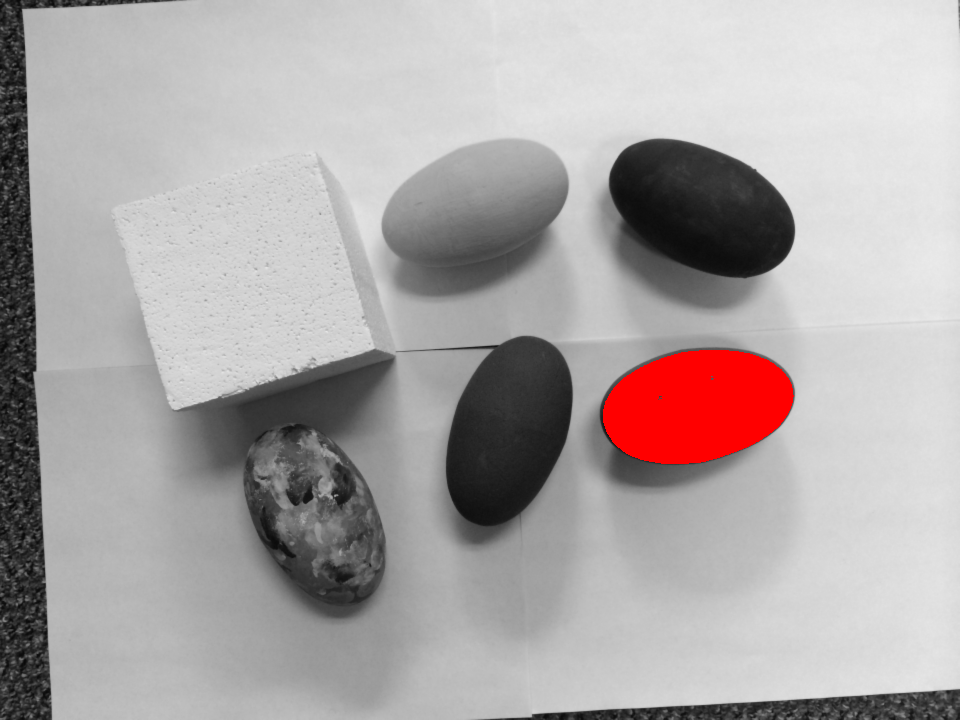
\includegraphics[width=140mm]{/Users/donj/workspace/cs585/Lab2/Mac/Assignment2/Data/greenEgg-result-0pt5-41.png}
\caption{greenEgg-result-0pt5-41.png}
\label{overflow}
\end{figure}

\begin{figure}[H]
\centering
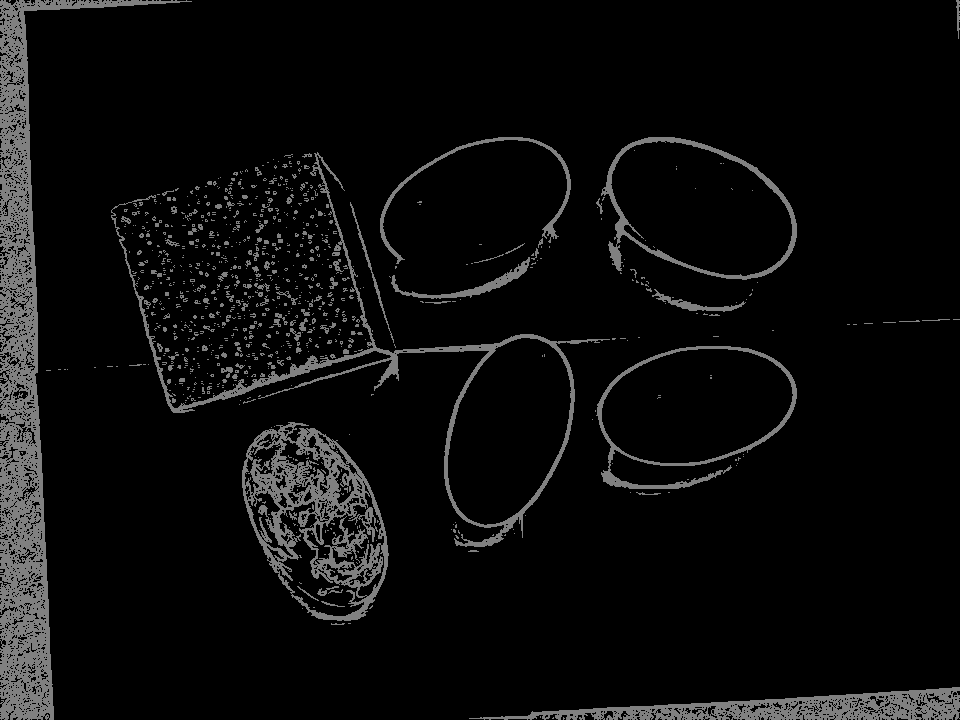
\includegraphics[width=140mm]{/Users/donj/workspace/cs585/Lab2/Mac/Assignment2/Data/blueEgg-edges-0pt5-42.png}
\caption{blueEgg-edges-0pt5-42.png}
\label{overflow}
\end{figure}

\begin{figure}[H]
\centering
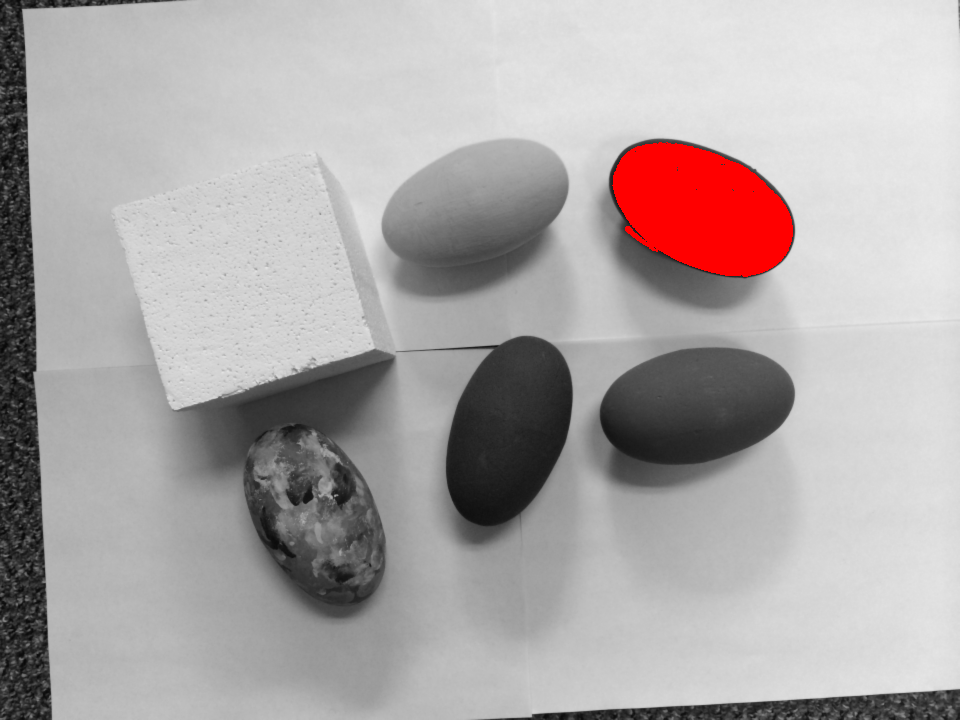
\includegraphics[width=140mm]{/Users/donj/workspace/cs585/Lab2/Mac/Assignment2/Data/blueEgg-result-0pt5-42.png}
\caption{blueEgg-result-0pt5-42.png}
\label{overflow}
\end{figure}

\item
Are you able to find any parameters that will allow you to identify the cube (or a face of the cube)? 

Harder with "gradient," because of the texture of the cube. Need low threshold and higher smoothing, however with "Canny" with dilation it is easy to select the same face on the cube cleanly (Smoothing sigma = 1.5, Canny thresholds = 20 and 60, Dilation kernel size = 3). See the results below (right vertical face):

\begin{figure}[H]
\centering
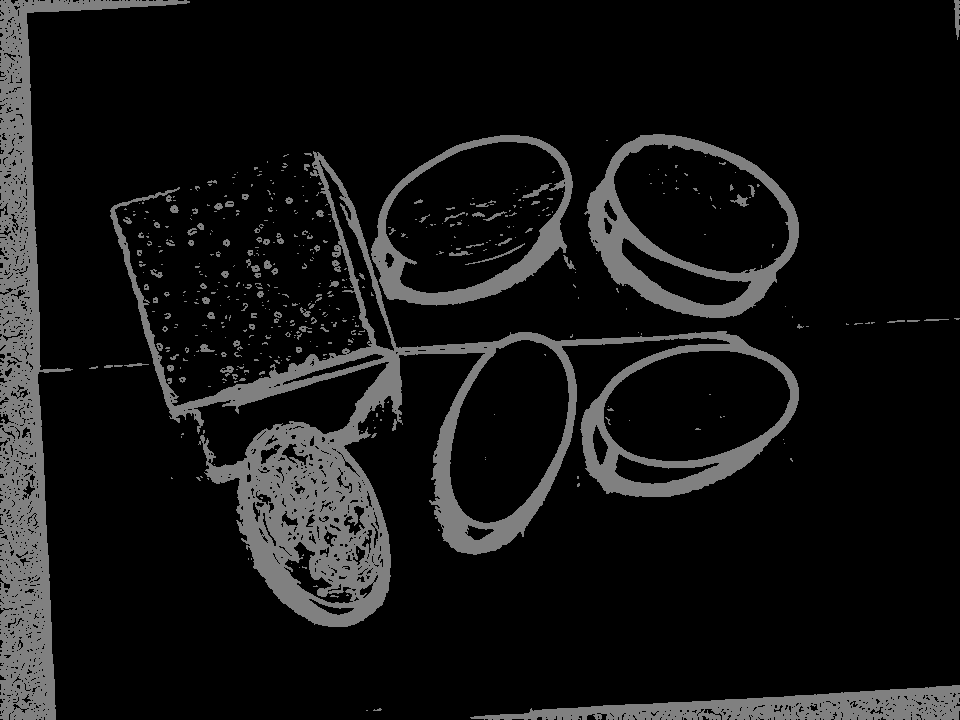
\includegraphics[width=140mm]{/Users/donj/workspace/cs585/Lab2/Mac/Assignment2/Data/cube-edges-1pt5-16.png}
\caption{cube-edges-1pt5-16.png}
\label{overflow}
\end{figure}

\begin{figure}[H]
\centering
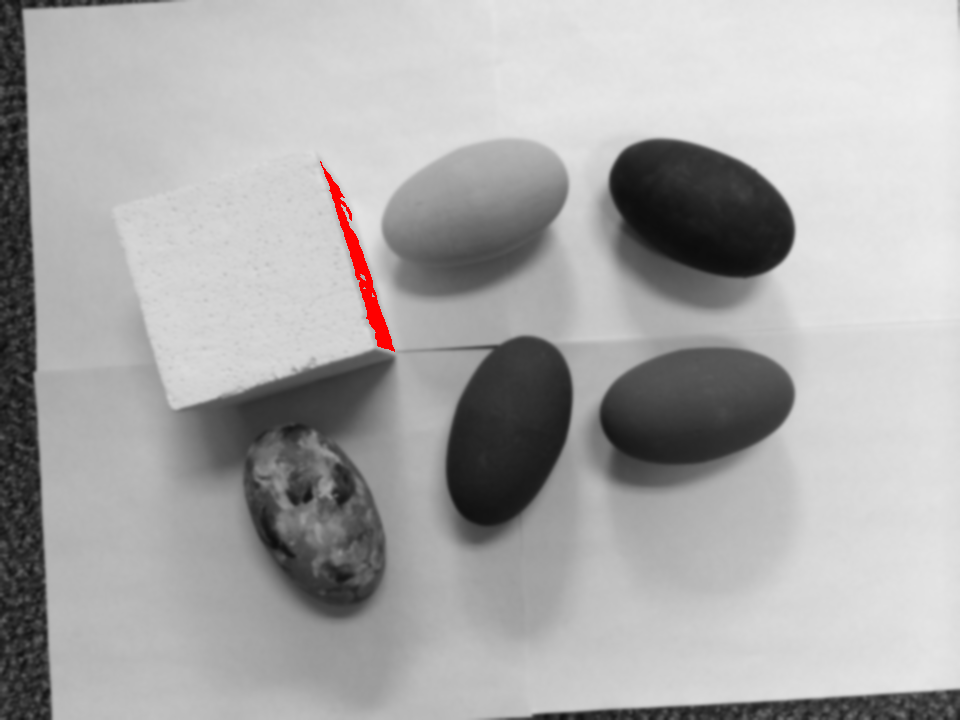
\includegraphics[width=140mm]{/Users/donj/workspace/cs585/Lab2/Mac/Assignment2/Data/cube-result-1pt5-16.png}
\caption{cube-result-1pt5-16.png}
\label{overflow}
\end{figure}

\begin{figure}[H]
\centering
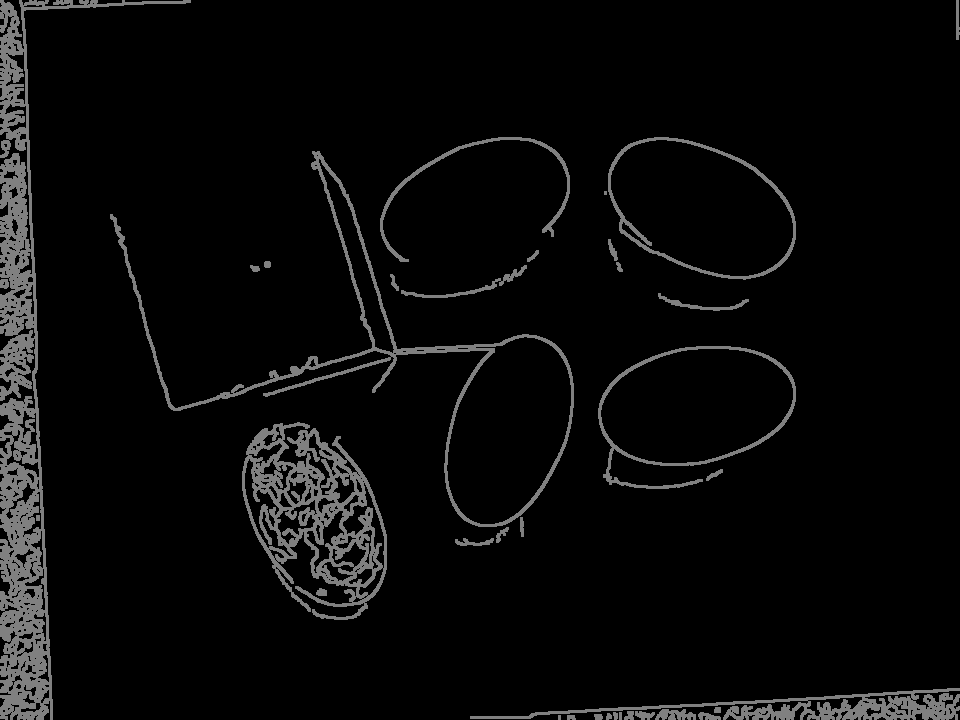
\includegraphics[width=140mm]{/Users/donj/workspace/cs585/Lab2/Mac/Assignment2/Data/cube-canny-dilation-edges.png}
\caption{cube-canny-dilation-edges.png}
\label{overflow}
\end{figure}

\begin{figure}[H]
\centering
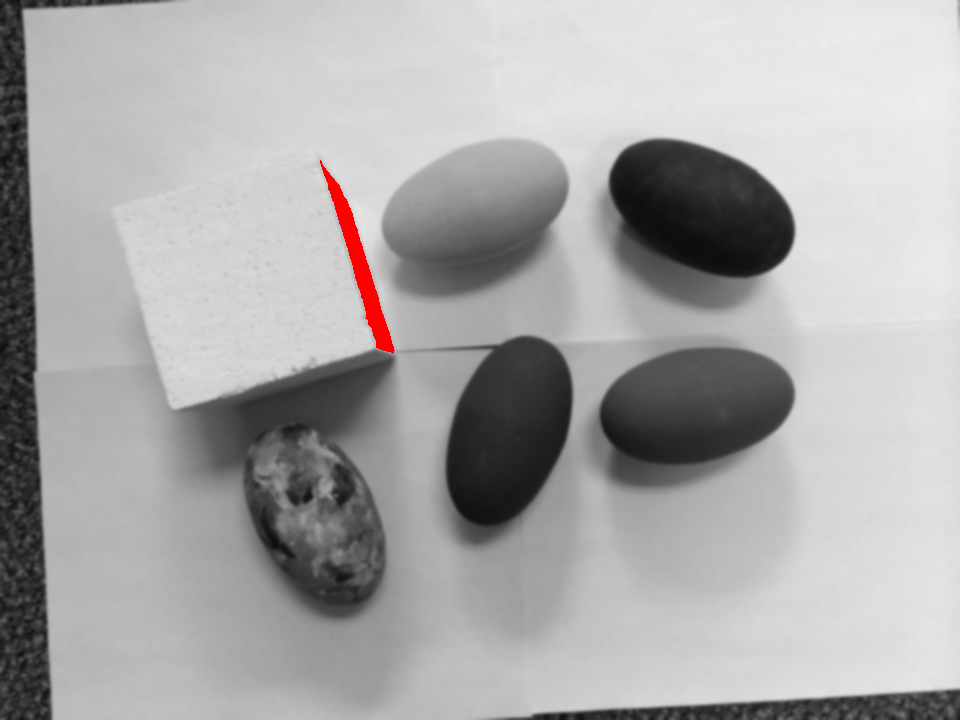
\includegraphics[width=140mm]{/Users/donj/workspace/cs585/Lab2/Mac/Assignment2/Data/cube-canny-dilation-result.png}
\caption{cube-canny-dilation-result.png}
\label{overflow}
\end{figure}

\pagebreak
\item
Use your program on the image "camoEggsOnPaper.jpg." If you knew that you were looking for textured objects on a plain background, what steps could you combine in order to highlight an entire egg, even though there are lots of internal edges? What type of binary image analysis steps could you perform in order to segment the entire egg? 

Canny with high thresholds (low=149 and high=447) and 3x3 kernel dilation can the closest to working. Nothing I tried to close off the eggs edges without almost filling the eggs with mask. Initial smoothing wasn't needed and didn't help for Canny, because Canny does a Gaussian smoothing as part of its procedure. Results below:

\begin{figure}[H]
\centering
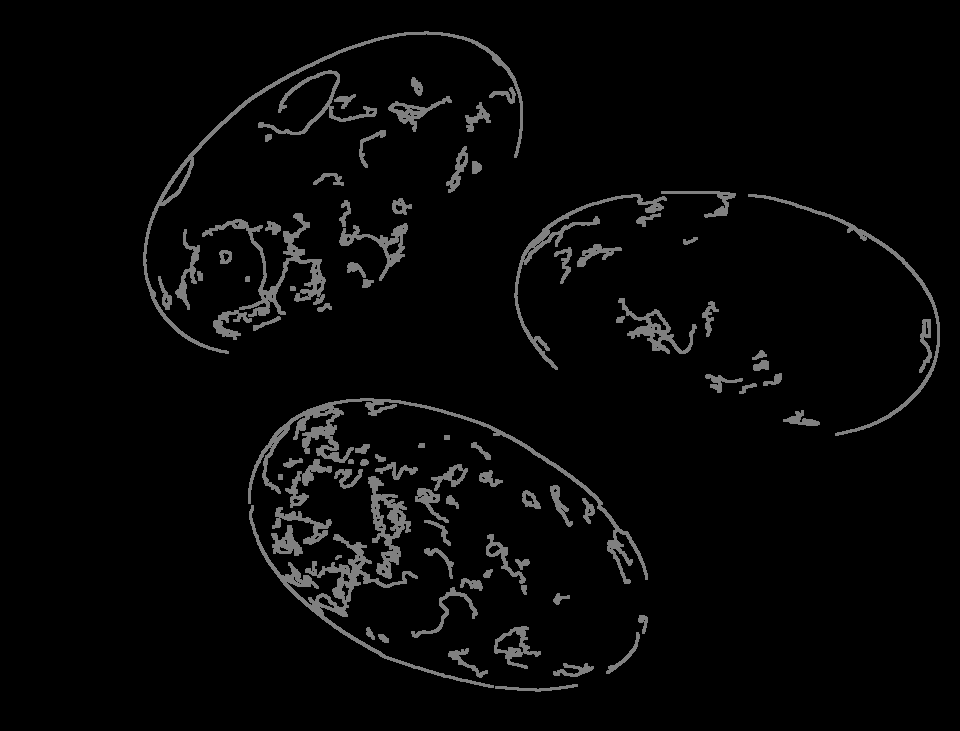
\includegraphics[width=140mm]{/Users/donj/workspace/cs585/Lab2/Mac/Assignment2/Data/camoEggsOnPaper-canny-dilation-edges.png}
\caption{camoEggsOnPaper-canny-dilation-edges.png}
\label{overflow}
\end{figure}


\item
Run your program on the image rainbowSpheres.jpg. You may find that some areas of the image are easier to segment than others. Try clicking on a few image regions (spots or stripes on the balls). Results below:

\begin{figure}[H]
\centering
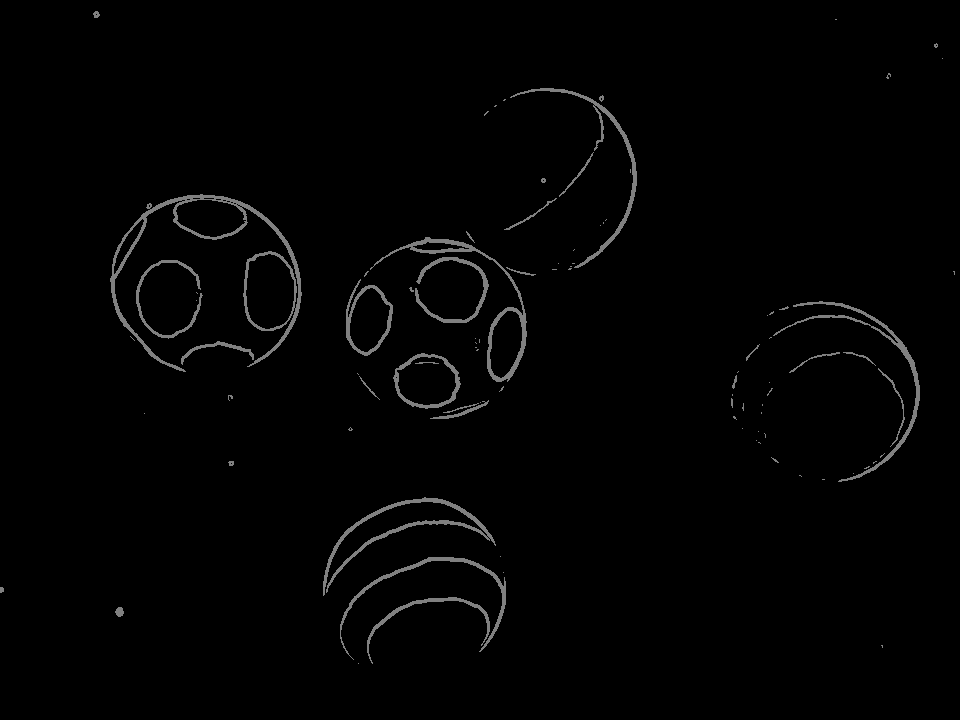
\includegraphics[width=140mm]{/Users/donj/workspace/cs585/Lab2/Mac/Assignment2/Data/rainbowEasy-edges-1-94.png}
\caption{rainbowEasy-edges-1-94.png}
\label{overflow}
\end{figure}

\begin{figure}[H]
\centering
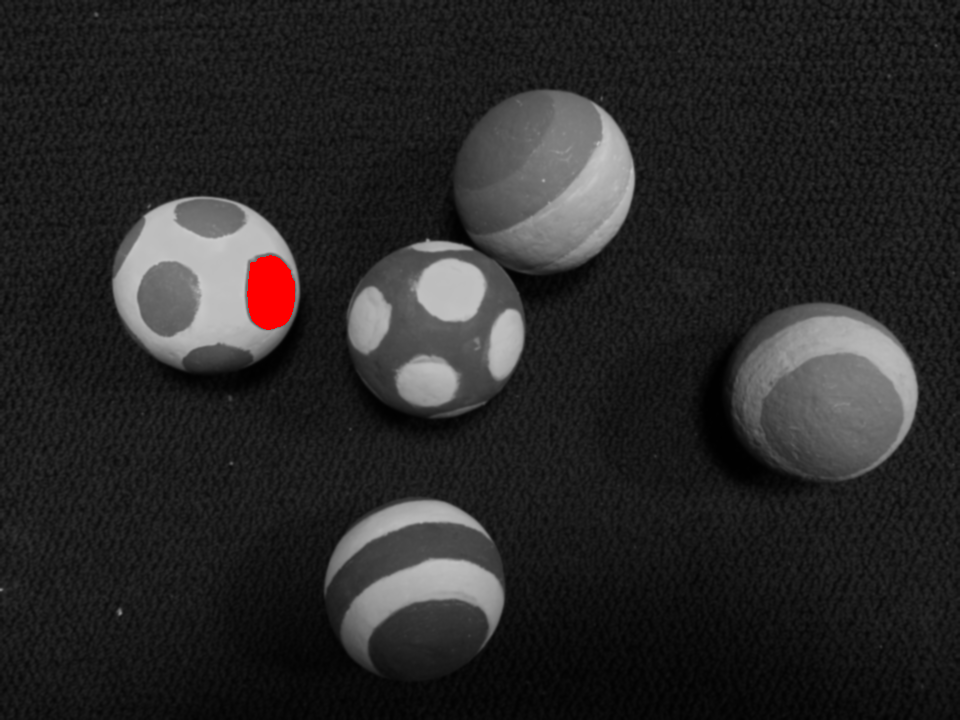
\includegraphics[width=140mm]{/Users/donj/workspace/cs585/Lab2/Mac/Assignment2/Data/rainbowEasy-result-1-94.png}
\caption{rainbowEasy-result-1-94.png}
\label{overflow}
\end{figure}


\item
Identify an area of the image that you think should be reasonably easy to pick out, but that the program is having trouble with. (For example, the purple and blue stripes on top of the rainbow ball). What is happening that causes the entire background to be filled when you attempt to fill the region bounded by edges starting in one of these areas?

The entire background is filled because the strip I picked out was missing part of its left edge.

\item
Use morphological operators to manipulate your edge map to help close gaps where the region-filling is leaking out so that you can fill in difficult region. Create before and after images of your troublesome regions. 

I used 1 sigma smoothing, a lower threshold and  a 3x3 kernel dilation to fill the gap. Results below:

\begin{figure}[H]
\centering
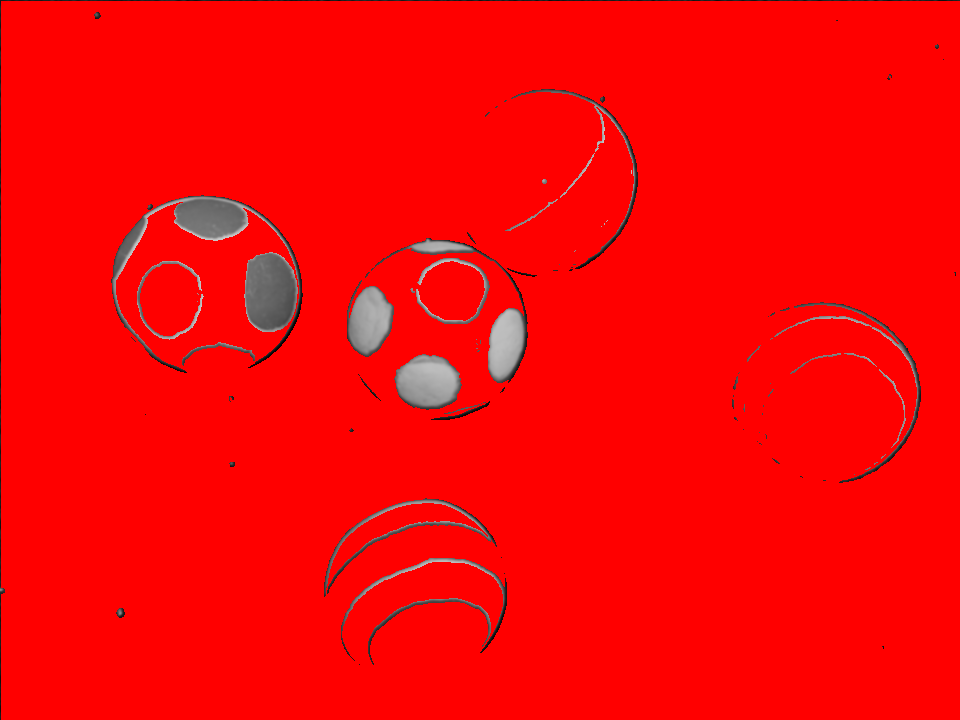
\includegraphics[width=140mm]{/Users/donj/workspace/cs585/Lab2/Mac/Assignment2/Data/rainbowHard-before-result-1-94.png}
\caption{rainbowHard-before-result-1-94.png}
\label{overflow}
\end{figure}

\begin{figure}[H]
\centering
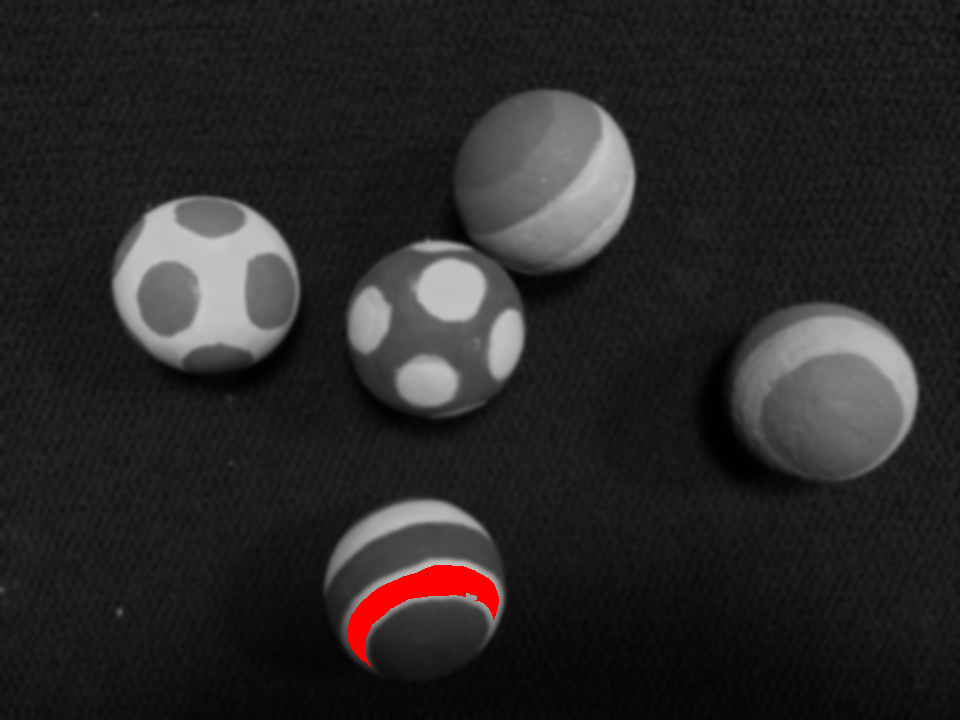
\includegraphics[width=140mm]{/Users/donj/workspace/cs585/Lab2/Mac/Assignment2/Data/rainbowHard-after-result-1-33.png}
\caption{rainbowHard-after-result-1-33.png}
;\label{overflow}
;\end{figure}

\end{enumerate}

\subsection{Lab Follow-up Questions (39 points)}
\begin{enumerate}

\item
Under the folder for Lab2, there is a folder called "gradients" containing several image where I have prepared several images using the gradient formula. Remember that the gradient of a function is just a vector containing the partial derivatives of the function with respect to each variable. You take a partial derivative of a function using the normal rules of calculus, but you treat all variables other than the one you are interested in as constants.


  \begin{enumerate}
    \item Write an expression for the gradient of I, given the formula that I used to generate the images.
    
    Holding y, \(\theta\) constant and taking the derivative with respect to x yields:
    
\begin{eqnarray*}
\frac{\partial I}{\partial x} I(x,y)=\cos \theta
\end{eqnarray*}    
    
        Holding x, \(\theta\)  constant and taking the derivative with respect to y yields:
    
\begin{eqnarray*}[H]
\frac{\partial I}{\partial y} I(x,y)=\sin \theta
\end{eqnarray*}    

    \item For each of three values calculate what you anticipate the values of the gradient will be:
\begin{eqnarray*}
\nabla I \left( \theta \right)=\left( \sin \theta, \cos \theta \right)
\\\nabla I \left( 0 ^{\circ} \right)=\left(0,1\right)
\\\nabla I \left( 45  ^{\circ} \right)=\left(\frac{\sqrt 2}{2},\frac{\sqrt 2}{2}\right)
\\\nabla I \left( 90  ^{\circ} \right)=\left(1,0\right)
\end{eqnarray*}    

	\item Using the program from the Lab, inspect the gradient of the images named "gradient_theta=0.png", "gradient_theta=45.png", "gradient_theta=90.png." Did you find any discrepancies? 
	\linebreak
	Yes, the 0 and ninety degree values were opposite of what I expected because the dI/dx and dI/dy values were reversed. These are the values I got from running the program against the three images: (1,0) , (0.7,0.7) and (0, 1).
	\item Using the program from the Lab, inspect the gradient of the image named "gradient_mysteryTheta.png." Report the values that you find and use them to determine the angle I used to generate the image.
	\linebreak
	Non-noisy mystery theta Arctan(dI/dy,dI/dx) = (255/191) = 53 degrees
	\item
	Histogram is gaussian before smoothing of mystery gradient noisy, using mean instead of three point gives Arctan(dI/dy,dI/dx) =  = (147.33/167.03) = 41.41 degrees
	\item 
	Histogram is just a few spikes after smoothing did seem to help much. Noisy mystery theta Arctan(dI/dy,dI/dx) = [(64+128+191)/(159+191+223)] = (383/573) = 56 degrees
	\item The image "gradient sigmoid.png" has been generated with such a function (given below). By inspecting the gradient of the image at the center point, estimate the angle that I used to generate the image.
	\linebreak
	The gradient looks like a a negative 45 degrees.
\end{enumerate}

\item Write down the kernel associated witth logic. It is a 9x9 kernel since there are nine terms:
\begin{tabular}{| l |c |r |}
\hline
1 &	2 &	1 \\
\hline
2 &	4 &	2 \\	
\hline
1 &	2 &	1 \\
\hline
\end{tabular}


	
\item
This code snippet below demonstrates the strange thing that is happening in when we add 1 to a color channel of an image. If the color channel is saturated (equal to 255) for a particular pixel, the color channel value rolls over to 0 because it is a unsigned byte. This why the more saturated areas of the image showed a strange speckled effect. The color also changes. For example if you add one to a saturated green channel in a  yellow pixel, the pixel changes to red.
\newline\newline
Here is the code and output:
\begin{lstlisting}
unsigned char nvar = 253;
for(int i=0;i<5;i++){
    printf("nvar + 1: %d\n", (unsigned int)++nvar);
}
\end{lstlisting}

Output:
\newline
nvar + 1: 254
\newline
nvar + 1: 255
\newline
nvar + 1: 0   (Here is where the value rolled over)
\newline
nvar + 1: 1
\newline
nvar + 1: 2

\end{enumerate}

\section{Lecture preparation}
\subsection{Preparation for Lecture 2}
\begin{enumerate}
\item
Formula for the area A, of the base of a cone, given an apex angle \( \alpha \), and height h:
\begin{eqnarray*}
\tan \alpha =\frac{r}{h}
\\r=h \tan\alpha
\\A=\pi r^{2}
\\A=\pi\left ( h\tan\alpha \right )^{2}
\end{eqnarray*}

\item
Solving for side Z of the blue triangle using properties of similar triangles:
\begin{eqnarray*}
\frac{Z}{f}=\frac{X}{u}
\\Z=\frac{X}{u}\cdot f
\\Z=\frac{5000 mm \cdot 25 mm}{0.540 mm}
\\Z=231.48m
\end{eqnarray*}

\item
Solving for side u of the red triangle using properties of similar triangles:
\begin{eqnarray*}
\frac{Z}{f}=\frac{X}{u}
\\u=\frac{f}{X}\cdot Z
\\u=\frac{25 mm \cdot 1000 mm}{10000 mm}
\\u=2.5 mm
\end{eqnarray*}

\item
Count N in pixels of u in for an \(18 \mu m\) pixel is:
\begin{eqnarray*}
N=\frac{u}{pixels\:size\:in\:\mu m}
\\N=\frac{2500 \mu m}{18 \mu m}
\\N=139 pixels
\end{eqnarray*}

\item
The magnitude of the vectors, n, v:
\begin{eqnarray*}
\left | n \right |=\sqrt{\left( 1\right )^{2}+\left( 1\right )^{2}}=\sqrt{2}
\\\left | v \right |=\sqrt{\left( 1\right )^{2}+\left( 0.5\right )^{2}}=\frac{\sqrt{5}}{2}
\end{eqnarray*}
\newline
The corresponding unit vectors \(\left \| n \right \|, \left \| v \right \|\):
\begin{eqnarray*}
\left \| n \right \|=(\frac{1}{\sqrt{2}},\frac{1}{\sqrt{2}})
\\\left \| v \right \|=( \frac{2}{\sqrt{5}}, \frac{1}{\sqrt{5}} )
\end{eqnarray*}

\item
The dot product of unit vectors \(\left \| n \right \|, \left \| v \right \|\):
\begin{eqnarray*}
\left \| n \right \|\cdot \left \| v \right \|=\frac{1}{\sqrt{2}}\cdot\frac{2}{\sqrt{5}}+\frac{1}{\sqrt{2}}\cdot\frac{1}{\sqrt{5}}
\\\left \| n \right \|\cdot \left \| v \right \|=\frac{3}{\sqrt{10}}
\end{eqnarray*}

\item
The angle \(\theta\) between vectors n, v:
\begin{eqnarray*}
\cos \theta=\frac{n \cdot v}{\left | n \right | \cdot \left | v \right |}
\\\cos \theta=\frac{1\cdot1+1\cdot\frac{1}{2}}{\sqrt{2}\cdot\frac{\sqrt{5}}{2}}
\\\cos \theta=\frac{3}{\sqrt 10}
\\\theta=18.44^{\circ}
\end{eqnarray*}

\item
The projection p of v, onto n:
\begin{eqnarray*}
p=\left | v \right |\cos \theta\cdot\left \| n \right \|
\\p=\frac{\sqrt{5}}{2}\cdot\frac{3}{\sqrt 10}(\frac{1}{\sqrt{2}},\frac{1}{\sqrt{2}})
\\p=\frac{3}{2\sqrt 2}(\frac{1}{\sqrt{2}},\frac{1}{\sqrt{2}})
\\p=(\frac{3}{4},\frac{3}{4})
\end{eqnarray*}


\item
The perpendicular vector q, between v and n:
\begin{eqnarray*}
q=v-p
\\q=(1,\frac{1}{2})-(\frac{3}{4},\frac{3}{4})
\\q=(\frac{1}{4},-\frac{1}{4})
\end{eqnarray*}
Finally, r equals the sum of the components we just calculated:
\begin{eqnarray*}
r=p+q
\\r=(\frac{3}{4},\frac{3}{4})+(\frac{1}{4},-\frac{1}{4})
\\r=(\frac{1}{2},\frac{1}{2})
\end{eqnarray*}

\end{enumerate}

\subsection{Preparation for Lecture 3}
\begin{enumerate}
\item
Adapted from source: http://www.csl.mtu.edu/cs2321/www/newLectures/26_Depth_First_Search.html

\begin{lstlisting}
Definitions: 
G is a graph
G.incidentEdges(v) - all of the edges associated with vertex v
G.opposite(v,e) - a vertex at the other end of edge e connected to v

Note: Every edge and vertex is marked initially as unexplored.
The algorithm terminates when all vertices and edges have been explored.
The initial vertex is the root.

Algorithm for depth-first, recursive transversal of graph G:

DFS(graph G, Vertex v) 

for all edges e in G.incidentEdges(v) do

    if edge e is unexplored then
    
        w = G.opposite(v, e) 
        if vertex w is unexplored then 
            label e as discovery edge 
            recursively call DFS(G, w) 
        else 
            label e as a back edge
            
\end{lstlisting}

\item
Algorithm to find connected components of graph and using depth-first transversal algorithm in previous question:
\begin{lstlisting}
Given a set of vertices {a,b,c,d,e,...}

Create a 2-dimensional matrix where the row and columns are the labeled with the vertices.
A cell value of 1 means they are connected and 0 unconnected.
Initialize (a,a), (b,b),(c,c).... equal to 1 - every vertex is connected to itself.

for all vertices v in G
	Do DFS(G, v) only for sum of row and column with same label is greater than one
		
		for each v, treated as root vertex, set connection matrix cell (v,v1), (v,v2), (v,v3) equal to 1 when v1, v2, v3, ... are visited during algorithm. 	
\end{lstlisting}

\pagebreak
\item
\begin{figure}[ht!]
\centering
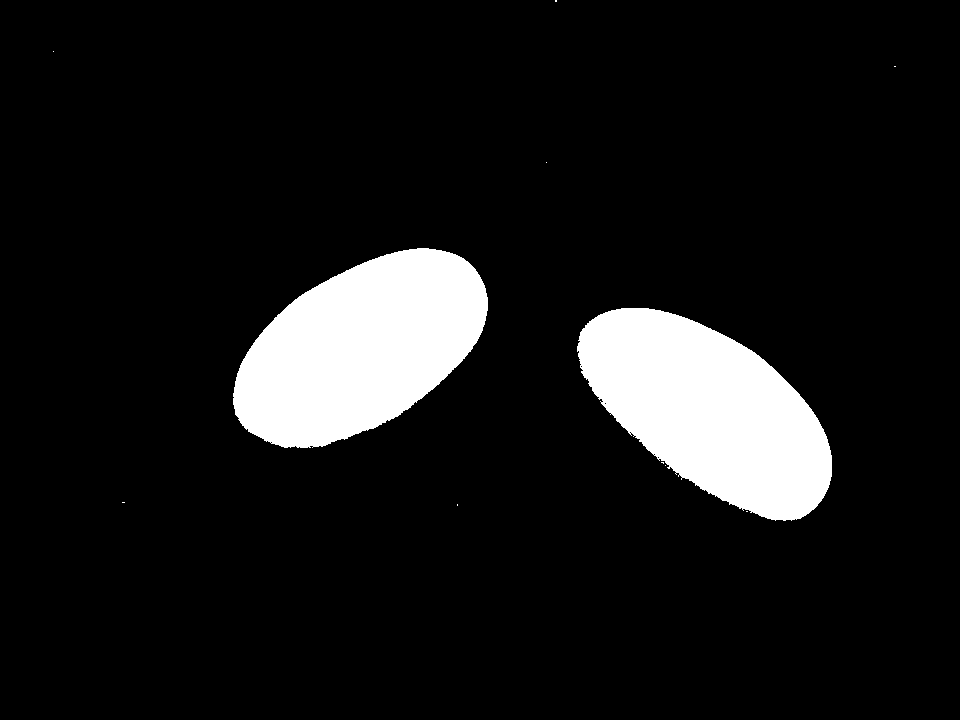
\includegraphics[width=100mm]{twoRedEggsThresholded175.png}
\caption{Results from running my program from section 1.2 on the picture "twoRedEggs.jpg"}
\label{overflow}
\end{figure}

\item
\begin{itemize}
\item
To find the number of red objects, I would define red for a pixel as a minimum ratio between the red channel and the blue, green channels
\item
Create a mask of all of those pixels defined as red, setting them equal to 1 and all other pixels equal to 0
\item
Run a depth first algorithm against the mask, visiting only the pixels equal to 1, treating each pixel as a vertex and each pixel boundary as an edge. Make it a greedy algorithm, collecting sets of connected pixels and keeping track of which pixels have been visited.
\item
Count the pixel sets to determine number of red objects
\end{itemize}
\item
My strategy for discarding the small extra regions that may pass through your red-object detector would be to require a minimal set size when counting the sets in the last step of the algorithm outlined in the previous question.

\item
If I was trying to create an rordered list of pixels that comprised the perimeter of an image region, for example, one of the red objects in the previous problem, I would:
\begin{itemize}
\item
Assume a x,y coordinate system for the image with (0,0) being the upper-left hand coordinate and both x and y increasing as you went down and to the right of the image.
\item
Find a pixel in one of the objects pixels sets from the previous problem with a value equal to 1 and having an x-coordinate minima in the set of pixels for that object. This will be one of the far left pixels in the object.
\item
Check for neighbor pixels with a value of one in this order: left, left-up, up, right-up, right, right-down, down, left-down
\item
When a non-zero neighbor is found, add it to a linked list, mark the pixel as visited and repeat the left to clockwise search pattern starting at the pixel boundary at which you entered.
\item
Repeat the process until you return to the first pixel where you started. The approach is similar to the approach used by bright physician from Egypt on the Maze of the Minotaur. The linked list contains the boundary pixels for the object.
\end{itemize}

\end{enumerate}

\end{document}
